\section{Auswertung}
\label{sec:Auswertung}

Nach der Messung werden die Filmstreifen ausgemessen. Dies geschieht aufgrund von fehlenden Werkzeugen mit einem gemeinen Lineal. Der systematische Fehler wird dabei auf $\pm\SI{1}{mm}$ gesetzt. Gemessen wird der Abstand zwischen zwei Linien, also der Kegelradius. Unter Betrachtung des gesamten Umfang des Filmstreifens wird schnell klar, dass ein Abschnitt des Umfangs des Filmstreifens gemessen wird. Das Verhältnis von dem Winkel $4\theta$ zu dem Abschnitt des Umfangs ist dabei gleich.
\begin{equation}
	\frac{4\theta}{2\pi} = \frac{s}{2\pi\cdot R}
\end{equation}
$R$ bezeichnet den Kammerradius und $s$ den gemessenen Radius der Kegel. Daraus folgt für den Winkel 
\begin{equation}
	\theta = \frac{1}{4}\frac{s}{R}.
\end{equation}
In Tabelle \ref{tab:KegelMetall} sind die gemessenen Kegelradien und die zugehörigen Winkel für Metall zu sehen. In Tabelle \ref{tab:KegelSalz} entsprechendes für Salz.
%
\begin{table}[h]
\centering
\caption{Kegelradien gemessen an den Filmstreifen umgerechnet in den Winkel $\theta$ für Metall.}
\label{tab:KegelMetall}
\begin{tabular}{c c | c c}
		\hline
		\multicolumn{2}{c|}{Vorne} & \multicolumn{2}{c}{Hinten}\\
		\hline
		\text{Kegelradius $s$ [m]} & \text{Winkel $\theta$} & \text{Kegelradius $s$ [m]} & \text{Winkel $\theta$} \\
		\hline
		0,065\pm0,001 & 0,284\pm0,004 & 0,045\pm0,001 & 1,213\pm0,004 \\
		0,098\pm0,001 & 0,428\pm0,004 & 0,065\pm0,001 & 1,287\pm0,004 \\
		0,115\pm0,001 & 0,502\pm0,004 & 0,082\pm0,001 & 1,374\pm0,004 \\
		\hline
\end{tabular}
\end{table}
%
\begin{table}[h]
\centering
\caption{Kegelradien gemessen an den Filmstreifen umgerechnet in den Winkel $\theta$ für Salz.}
\label{tab:KegelSalz}
\begin{tabular}{c c | c c}
		\hline
		\multicolumn{2}{c|}{Vorne} & \multicolumn{2}{c}{Hinten}\\
		\hline
		\text{Kegelradius $s$ [m]} & \text{Winkel $\theta$} & \text{Kegelradius $s$ [m]} & \text{Winkel $\theta$} \\
		\hline
		0,028\pm0,001 & 0,122\pm0,004 & 0,015\pm0,001 & 1,213\pm0,004 \\
		0,040\pm0,001 & 0,172\pm0,004 & 0,031\pm0,001 & 1,235\pm0,004 \\
		0,048\pm0,001 & 0,207\pm0,004 & 0,041\pm0,001 & 1,265\pm0,004 \\
		0,056\pm0,001 & 0,244\pm0,004 & 0,052\pm0,001 & 1,289\pm0,004 \\
		0,063\pm0,001 & 0,273\pm0,004 & 0,057\pm0,001 & 1,322\pm0,004 \\
		0,075\pm0,001 & 0,327\pm0,004 & 0,065\pm0,001 & 1,346\pm0,004 \\
		0,000\pm0,001 & 0,000\pm0,000 & 0,070\pm0,001 & 1,392\pm0,004 \\
		0,000\pm0,001 & 0,000\pm0,000 & 0,077\pm0,001 & 1,438\pm0,004 \\
		0,000\pm0,001 & 0,000\pm0,000 & 0,082\pm0,001 & 1,506\pm0,004 \\
		\hline
\end{tabular}
\end{table}
%
Mit den bestimmten Winkeln und Gleichung (\ref{eq:Struk2}) kann nun die Strukturamplitude für verschiedene Netzebenen und damit verschiedene $[hkl]$-Werte bestimmt werden.

\subsection{Systematische Fehler}

Als Erstes ist darauf hinzuweisen, dass durch den Versuchsaufbau zwei systematische Fehler gemacht werden, die wie folgt in die Auswertung einfließen.
Die Systematischen Fehler entstehen bei den Ringradien. 
Dabei entsteht der Eindruck, dass die Gitterkonstante a abhängig von dem Beugungswinkel $\theta$ ist. \\
Der erste systematische Fehler liegt in der Messung von dem 4 $\theta$-Winkel, der stets zu groß gemessen wird. 
Problematisch ist das so kleine Winkel große Fehler besitzen. 
in Abbildung \ref{fig:sys1} wird schematisch gezeigt, wie das wahre $\theta$ aussehen sollte.
\begin{figure}
\centering
	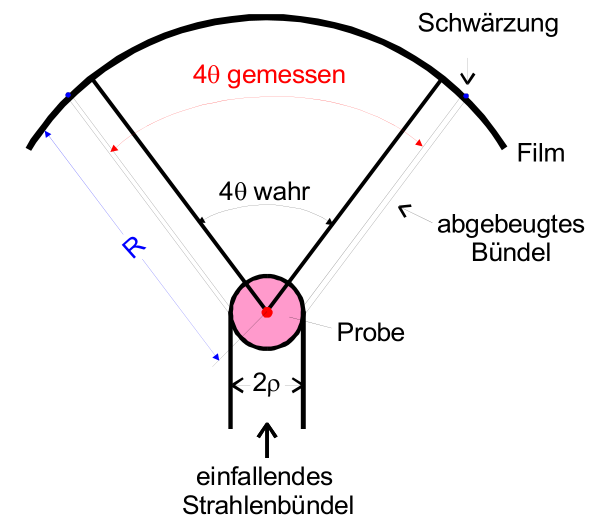
\includegraphics[width = 0.5\textwidth]{Abbildungen/Syst1.png}
	\caption{Darstellung des systematischen Fehlers, der aus der Absorbtion innerhalb des Probenstäbchens entsteht \cite{Anleitung}.}
	\label{fig:sys1}
\end{figure} 
Das Problem liegt darin, dass der Großteil der Strahlung komplett absorbiert wird und nur am Rand Beugungseffekte entstehen die aus der Probe kommen.
Berücksichtigt wird dies durch die Korrektur $\Delta a_A$ nach Bradley und Jay in Gleichung \ref{eq:syst1}.
\begin{equation}
\frac{\Delta a_A}{\text{a}} = \frac{\rho}{2\text{R}}\left( 1-\frac{\text{R}}{\text{F}} \right)\frac{\cos^2{\theta}}{\theta}
\label{eq:syst1}
\end{equation}
Der Größen sind in der Abbildung \ref{fig:sys1} dargestellt. 
$\rho$ ist der Radius des Probenstäbchens, R der Kameraradius und F der Abstand zwischen Fokus und Probe.
Dieser Fehler führt in dem Plot von $a(\theta)$ gegen $\cos^2{\theta}$ zu den Fehlerbalken in a.
\\\\
Der Zweite Systematische Fehler resultiert aus der Geometrie des Aufbaus.
In der Regel sind die Achse des Probenzylinders und die Achse des Films leicht gegeneinander verschoben. 
Das ist in Abbildung \ref{fig:sys2} dargestellt.
\begin{figure}
\centering
	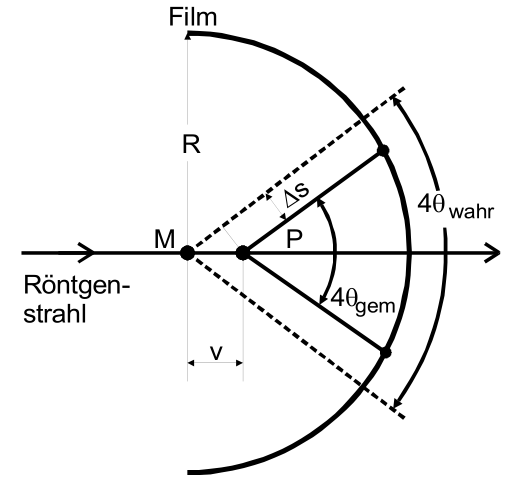
\includegraphics[width = 0.5\textwidth]{Abbildungen/Syst2.png}
	\caption{\cite{Anleitung}.}
	\label{fig:sys2}
\end{figure}
Dieser Fehler wirkt sich wieder auf das gemessene $\theta$ aus und ergibt die Abweichung $\Delta \theta$ wie in Gleichung \ref{eq:syst2} aufgeführt ist.
Der Abstand $\Delta$S und die Verschiebung v sind aus der Skizze \ref{fig:sys2} zu entnehmen.
\begin{align*}
\Delta \text{S} &  = -\text{v} \sin{2 \theta} \\
\Delta \theta & = -\frac{\Delta \text{S}}{2\text{R}}
\end{align*}
\begin{equation}
\Delta \theta = \frac{\text{v}}{2\text{R}}\sin{2\theta} = \frac{\text{v}}{\text{R}}\cos{\theta}\sin{\theta}
\label{eq:syst2}
\end{equation}
Unter Berücksichtigung der differnzierten Bragg-Bedingung ergibt sich der Korrekturterm $\Delta a_v$ in Gleichung \ref{eq:system} aus
\begin{align*}
\frac{\Delta \text{a}}{\text{a}} = \frac{\Delta \text{d}}{\text{d}} = -\Delta \theta \frac{\cos{\theta}}{\sin{\theta}}.
\end{align*}
\begin{equation}
\frac{\Delta a_v}{\text{a}} = \frac{\text{v}}{\text{R}}\cos^2{\theta}
\label{eq:system}
\end{equation}
Das heißt, die Gesamte Abweichung der Gitterkonstante resultiert in $\Delta a_{ges}$, welche as der Summe der beiden systematischen Fehler $\Delta a_A$ und $\Delta a_v$. 
Dabei ist die Gitterkonstante $\Delta a_{ges}$ proportional zu $\cos2{\theta}$.\\
Die tatsächliche Gitterkonstante a ist deshalb aus dem y-Achsenabschnitt des Plots $a(\theta)$ gegen $\cos^2{\theta}$ zu entnehmen.

\subsection{Metall}